\chapter{Smart Grid Power Flow Status Monitoring}

The \acrshort{sg} consists of a vast number of both conventional and modern, more dynamic, production facilities, which requires thorough monitoring in order to ensure the optimal distribution of electrical energy. The requirement of a consistently stable and reliable supply of energy is constant, while the amount of energy demanded is dynamically changing according to the demand for power at any time. 

Therefore, the proper \acrlong{sg} operation might be considered virtually impossible without a  close monitoring of current power flow, as well as the ability to instantly adjust the supply of power according to present needs,  without the risk of causing power surges or blackouts. For this purpose, the Wide Area Monitoring System analyses the levels of electrical power as monitored by sensors, continuously sampled and forwarded to the \acrshort{wams}, through  a networked infrastructure continuously time-synchronised within a fraction of a second tolerance, for the less demanding subsystems.
The correctness of this time source is critical to the reliability, and therefore, the proper operation of the monitoring system, constituting the primary decision criteria for actions controlling the supply of power.




\section{Time Synchronisation}

In order to be able to synchronise events in time, it is mandatory to adjust the clock of each participating actor, analogous to the classic pre-operational physical watch-synchronisation meetings in the physical domain. 
The \acrshort{sg} time synchronisation requirements are, to say the least, a bit more demanding than a simultaneous(-ish) press on buttons to start timing from a common time reference.
Several articles, of which \cite{appasani2018review} may serve as an example, stresses the importance of utilising a precise and reliable times source.

%
  %Given the distributed nature of the \acrshort{pmu} devices providing samples from locations distributed over a Wide Area Network, the \acrfull{gps} is the  time source selected. 





\subsection[System Operations Benefits]{System Operations Benefits of proper Time Synchronisation}

In \cite{dagle2019importance}, \citeauthor{dagle2019importance} states the following aspects as the benefits for Smart Grid operation, of ensuring correct time synchronisation:


\begin{itemize}
    \item \textbf{Situational Awareness and Wide-Area Monitoring} The improved quality of Syncrophasor data makes life easier for system operators, getting a more detailed overview of system state. The real-time state of the monitoring data presented, enabled the operators to react proactively to any status issues, before the underlying system state is allowed to a potential system blackout.
    \item \textbf{Real-Time Operations} \acrshort{pg} system operators are using \acrlong{pmu} data in order to pinpoint potential locations possibly hosting faulty equipment, enabling the early remediation of a potential issue capable of disturbing proper grid operatuion.
    \item \textbf{Power System Planning} The more detailed situational awareness obtainable from the usage of Synchrophasor data, gives the grid system operators a tool which enables them to ensure the optimal power asset utilisation, while at the same time being able to improve \acrlong{se} systems, explained in Section \ref{sec:3-SE}, as well as testing for compliance standards.
    \item \textbf{Forensic Event Analysis} In the case of black-outs and other disturbance events, the availability of fine-grained Synchrophasor data, time-stamped to $\mu$-second accuracy, be a good tool for any post-event investigations aiming to conclude on the events leading to the event to be investigated.
    
\end{itemize}

\subsection{Possible effects of Time Synchronisation Data Impairment}

In \Cite{martin2019impact}, \citeauthor{martin2019impact} lists a number of side-effects which could result form the absence of high-quality data material from the \acrshort{wams}.


\begin{itemize}

    \item \textbf{Data loss} due to delayed, or otherwise erroneous, transmission of Syncrophasor data from the \acrshort{pdc}s and \acrshort{pmu}s covered in the previous chapter, will pprevent the \acrshort{wams} from obtaining a correct snapshot og the current System State at any time. The missing data will give the operators system state information that is incomplete, and possibly erroneous,  on which to base their actions in order to cope with possible system state issues.
    \item \textbf{Data corruption} causes the \acrshort{wams}, and ultimately the grid operators, to be unable to interpret the affected data in any meaningful way, possibly loosing valuable system information. Data corruption could occur at any stage of the transmission from the sensors, caused by sensor malfunction, via the \acrshort{pdc}s and, indeed, even by some issues with the proper phasor calculation at the \acrfull{pmu}.  
    \item \textbf{Inaccurate representation} of engineering quantities like specialised \acrshort{pg} networking equipment like transducers, or devices used to record or display the data. The inaccuracy could be caused by wrong scaling or timing, as well as interference and noise. 
    \item \textbf{Lack of precision}, will render the available data less useless for monitoring purposes, when compared with a situation of receiving data of sufficient precision. The lack of precision negatively affects data accuracy, which may ultimately result in a situation where the operators may have an inaccurate situation stare awareness. The possible situation of added noise which could be a result of increasing the precision is not relevant for Syncrophasor data not containing a significant level of noise.
    \item \textbf{Incorrect identification} of measurements could be caused by the wrong labeling of any sensors to be used in order to monitor any equipment located in the \acrshort{pg}. Incorrect data identification could also be an issue caused by a Syncrophasor data  having erroneous identifiers of any related equipment.
    \item \textbf{Excessive or inconsistent latency} may cause the various system components, to fail to provide the data required in order to ensure displaying the proper system state to some part, or application, residing in the \acrlong{wams}. 
\end{itemize}




%\subsection[Smart Grid Time Sync Precision Requirements]{Smart Grid Time Synchronisation Precision Requirements}

%In order to ensure the time precision required for the \acrshort{sg}, the correct selection of time synchronisation mechanisms is vital. 





\subsection{WAMS Time Synchronisation}



The \acrlong{wams} is critically dependant on precise Time Synchronisation, as a Time Synchronisation error of a few $\mu$-seconds may result in \acrshort{sg} monitoring instability. The time stamps produced by Synchrophasors, pinpointing the exact time of any system event, is vital in order to ensure precise and reliable system state information.
In the event of a system alert being triggered by erroneous system state Information, corrective actions by operators might have undesired effects. In order to synchronise the samples received from the \acrshort{pmu}, the \acrshort{pdc}, as well as the \acrshort{pmu} devices producing the samples, is vitally dependant on precise timing adjustments, in order to establish a precise and correct overview of system state. Incorrect synchronisation of measurements caused by erroneous timing information, will produce an equally wrong system state overview, as presented in the \acrshort{sg} \acrshort{wams}.

\begin{figure}[t]
\includegraphics[width=\textwidth]{figures/phasorMaeasuremantSystemsNF.png}

\caption[Phasor Measurement Systems]{Phasor Measurement Systems, as presented in 

\cite{johnson2018standards} Slide 3

}
\label{fig:PhasorMeasurementSystems}
\end{figure}



\section{Protocols}
A large number of protocols are defined, in order to standardise the operation of the \acrlong{sg}.
Figure \ref{fig:PhasorMeasurementSystems} provides an overview of standards relevant for the specified areas relevant for the Phasor Measurement System.
Of these, I will focus mainly on a couple of protocols, seen in the upper left part of the figure:
\begin{itemize}
    \item For the protocols in the timing standards, my main focus will be on the \acrfull{ptp} standard, IEEE 1588.
    \item for the protocols in the communications standards, my main focus will be on the Synchrophasor standard IEEE c37.118.2\footnote{For the IEEE C37.118 revision of 2011, the standard IEEE c37.118 was separated in two parts.\\ IEEE c37.118.1 standardises communications, whereas IEEE c37.118.2 standardises measurements.}
\end{itemize}
 In my thesis, concerning \acrlong{tda}s, I am going to focus on the IEEE 1588 protocol, used in order to provide time synchronisation of devices residing in a \acrlong{ptp}-enabled network, supported by \acrshort{pmu}s not\footnote{PTP are now common in recent years as an alternative to GPS for PMU time synchronisation.} relying on \acrfull{gnss} systems, like the \acrfull{gps} for time synchronisation.
%\cite{2021arXiv210311657E} \hl{describes communication protocols} in the  \acrshort{sg}.













\section{Time Synchronisation Protocols}


Time Synchronisation protocols are used in order to synchronise the time of interconnected devices in need of synchronised time for various purposes. In the case of synchrophasor devices, the devices needs to be time synchronised in order for \acrshort{sg} \acrshort{wams} operators to get a correct overview of the system state.

\subsection{Time Synchronisation Protocols Precision Requirements}
Time synchronisation protocols are controlling the synchronisation of time between various devices of the grid, like the \acrshort{pmu}s, collecting Phasor Measurements from a defined number of measuring devices. Synchronised time is crucial in order to ensure each PMU is able to put the correct time stamp on each Phasor Measurement, before transmitting the resulting Synchrophasor for each time stamp, to the destined PDC device.\\ 

In the event one of the Synchrophasors have an erroneous time stamp, an error affecting the integrity of the Synchrophasor data is introduced. As described in \cite{moussa2016security}, \acrlong{ptp} Synchronisation network
, as well as \acrlong{gnss} based synchronisation networks, are both capable of producing the precision required by the Synchrophasor protocols, as opposed to the more common \acrfull{ntp} commonly used in ordinary computer networks. As my thesis covers \acrshort{ptp} time synchronisation only, my description of time synchronisation protocols is limited to the \acrfull{ptp}.

%\subsection{Synchrophasor data alignment attack}
%Eq \ref{DMS} about DMS, and  eq \ref{DSM} about DSM.









%Unlike the \acrlong{cpg}, the \acrlong{sg} enables bidirectional flow of power, by customers operating micro grids enabling customers to sell excessive power back to the network.








%\section{Historical}
%SCADA monitoring flaws -> PMU




%\section{PMUs}
%PMU
%-  Descripton of PMU
%- phasor
%- synchronised phasors
%- Communication with PDC

%\section{PDCs}
%PDC
%- Collecting synchronised phasors from PMU
%- Grouping synchronised phasors with same timestamp into Synchrophasor record
%- At deadline, transmitting Synchronaised phasors, received before deadline.
%- Improved security. 
%\section{Synchrophasors}
%Synchrophasors
%- overview
%- sync precision requirements:
 
%\section{Protocols used for monitoring}
%Protocols
%- Figure from PowerPoint
%- Concentrating on upper left side of figure.


%- capabilities of x.2011 x=synchrophasor protocol

%PTP
%Rationale for concentrating on PTP
%Descriptino of the protocol
%Time synchronisation via PTP
%PTP delay attack (types)



\subsubsection{Precision Time Protocol services}
The \acrfull{ptp} is a network-based time protocol, enabling the time difference between devices to be synchronised within a fraction (in the order of a few $\mu$s) of a second, satisfying the requirements of the \acrshort{sg} \acrshort{wams} for the precise time synchronisation  ensuring the reliable and robust transmission of synchrophasors from the \acrshort{pmu} to the \acrshort{wams}. 
\subsubsection{Description of PTP time synchronisation}

A device, being synchronised  by the \acrshort{ptp} protocol, reads its system time from a clock which is continuously synchronised by a network of one or more slave clocks, being periodically synchronised via various types of hybrid\footnote{Hybrid clocks are a master clock for some clocks, while being a slave clock for others.} clocks, ultimately synchronised with a Grand Master Clock.\\ 

The time of the slave clock, is being adjusted according to the following process, as visualised in figure \ref{fig:PTP-timing-Diagram}, and described in \cite[p. 51]{Eidson2006}:


\begin{quotation}
    
   " The basic sequence in synchronizing a slave clock to a master clock is:
    \begin{itemize}
        \item The master clock sends a Sync message to all directly connected slave
clocks. The master clock generates a timestamp $t_1$ based on the master’s
local clock, indicating the Sync message sending time at the master clock.
\item A slave clock receives the Sync message and generates a timestamp $t_2$
based on the slave’s local clock, indicating the Sync message receipt time
at the slave.
\item The master clock communicates the Sync message sending timestamp $t_1$
to the slaves as a data field in a Follow Up message.
\item The slave clock sends a Delay Req message to the master clock. The slave
clock generates a timestamp $t_3$ based on the slave’s local clock, indicating
the Delay Req sending time at the slave clock.
\item The master clock receives the Delay Req message and generates a timestamp $t_4$ based on the master’s local clock, indicating the Delay Req receipt time at the master clock.
\item The master clock communicates the Delay Req receipt timestamp $t_4$ to
the slave as a data field in a Delay Resp message.
\item The slave uses the four timestamps $t_1$, $t_2$, $t_3$, and $t_4$ to compute the offset
between the slave and master clocks. "\cite[p. 51]{Eidson2006}
    
    \end{itemize} 
\end{quotation}


\begin{figure}[ht]
    \centering 
    \includegraphics[ width=\textwidth]{figures/PTP-timing-Diagram.png}
    \caption[Timing diagram for synchronization messages]{As presented in \cite[p. 51]{Eidson2006}: Timing diagram for synchronization messages.} 
    \label{fig:PTP-timing-Diagram} 
\end{figure}  


Following the message exchange visualised by \figureautorefname { } \ref{fig:PTP-timing-Diagram}, the Slave clock  uses the time offset $offset$ from the Master clock time, calculated by Equation \ref{eq:offset}, in order to synchronise with the Master clock. One fundamental 


\begin{equation} \label{eq:t1}
t_1 = t_0 + offset + d_1 
\end{equation}

\begin{equation} \label{eq:t3}
t_3 = t_2 - offset + d_2 
\end{equation}

\begin{equation}   \label{eq:d1}
d_1 = d_2 = d  
\end{equation}

%\textbf{Bla bla }Equation \ref{eq:t1}

\begin{equation}  \label{eq:offset}
offset = \frac{(t_2 - t_1) + (t_4 - t_3)}{2}
\end{equation}

In order to be able to achieve the time difference required, the \acrshort{ptp}, as described by  \citeauthor{Eidson2006}, in \cite{Eidson2006}, is dependant on:

\begin{itemize}
    \item Timestamped network events, messages, which is  used for synchronisation.
    \item A method of timestamp transmission as required for synchronisation.
    \item Overcoming any timing impairments introduced by system components.
\end{itemize}

As is discussed by several papers, including \cite{ullmann2009delay}, a vulnerability of \acrshort{ptp}, and similar protocols like the ``\acrshort{ntp} protocol, is the assumption given in equation \ref{eq:d1} of $d_1$ being equal to $d_2$, assuming symmetrical packet transmission delay delay between the Synchronisation target and the corresponding Synchronisation source.


\begin{figure} %[ht]
 
    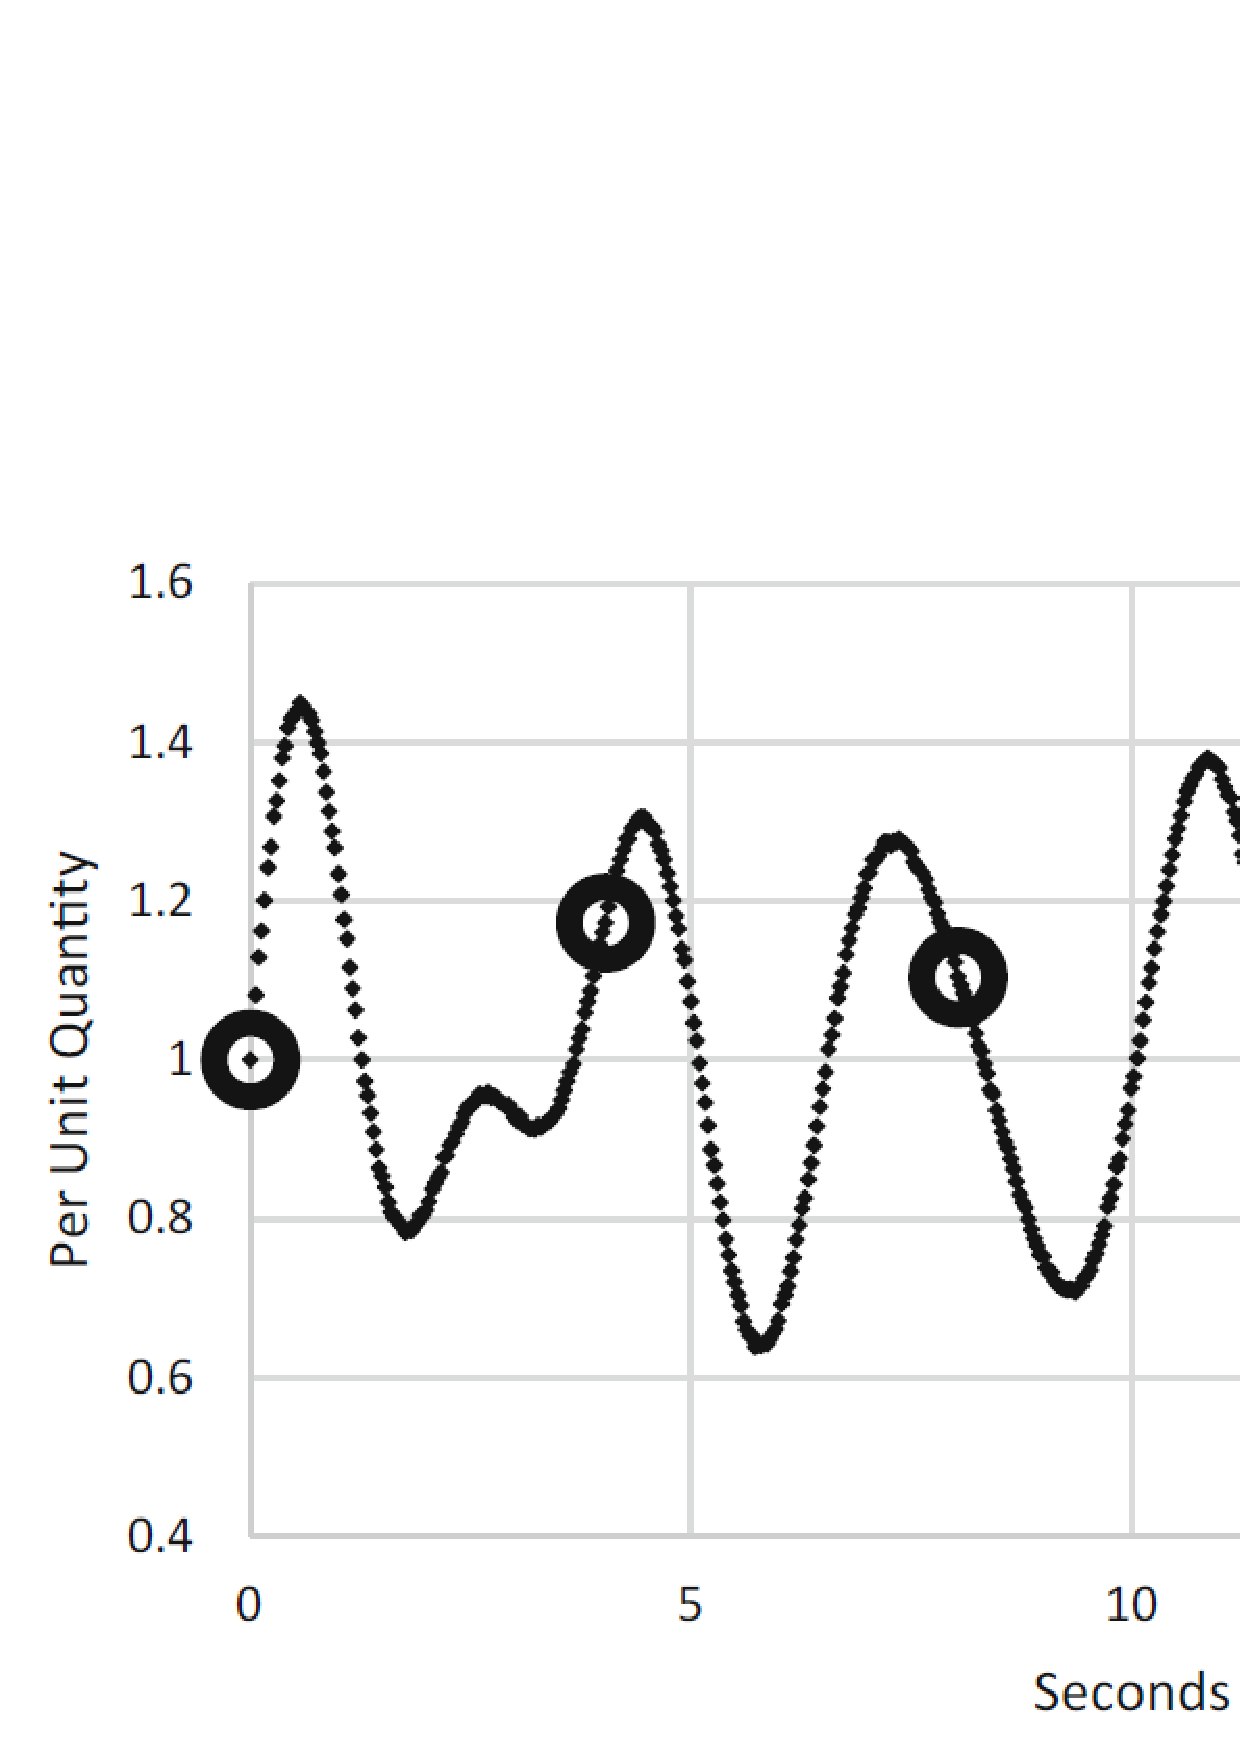
\includegraphics[ width=\textwidth]{figures/syncrophasors-vs-scada.png}
    \caption[Difference between Synchrophasor and SCADA measurements]{As presented in \cite[p. 3]{dagle2019importance}: Notional representation of the difference between synchrophasor and SCADA
measurement. Figure credit: \citeauthor{dagle2019importance}.} 
    \label{fig:syncrophasors-vs-scada}
\end{figure}  





\subsection{Synchrophasors}

A number of protocols has been developed and maintained, in order to standardise the format of the synchronised phasors to be transmitted, as well as the actual method of transmission used in order to transfer the standardised data.
The \acrshort{pmu} is receiving values from sensors, on which it is able to calculate voltage level and phase angle of the energy flow. It is utilising a time-source to pinpoint measurements in time, producing synchrophasors, to be transmitted to the nearest \acrshort{pdc}. 
As described in \cite{dagle2019importance}, the data received from traditional \acrshort{scada} systems are time-stamped after arriving at the control station. The synchrophasors of the \acrshort{wams} on the other hand are, as described in \cite{ali2016wide}, being time-stamped by the \acrshort{pmu} in real-time before being transferred to the control system. The sampling rate of the \acrshort{pmu}, results in synchrophasor data enabling operators of the \acrshort{wams} to get real-time visualisation of critical elements, like the state of energy flow  of the \acrlong{sg}. The increased granularity of the measurement system allows for the detection of anomalies undetectable by traditional \acrshort{scada} systems, as illustrated by \figureautorefname { }\ref{fig:syncrophasors-vs-scada}. 
The increased sampling rate, of the synchrophasors of the \acrshort{wams} systems enables a more fine-grained view of energy distribution system state changes. However, in order for the \acrshort{wams} system to get the correct system state information, correct time stamps is critical. 
Therefore, the time-synchronisation mechanisms of the \acrshort{pmu} system is of critical importance. \\ 

\begin{figure}
    \centering {
    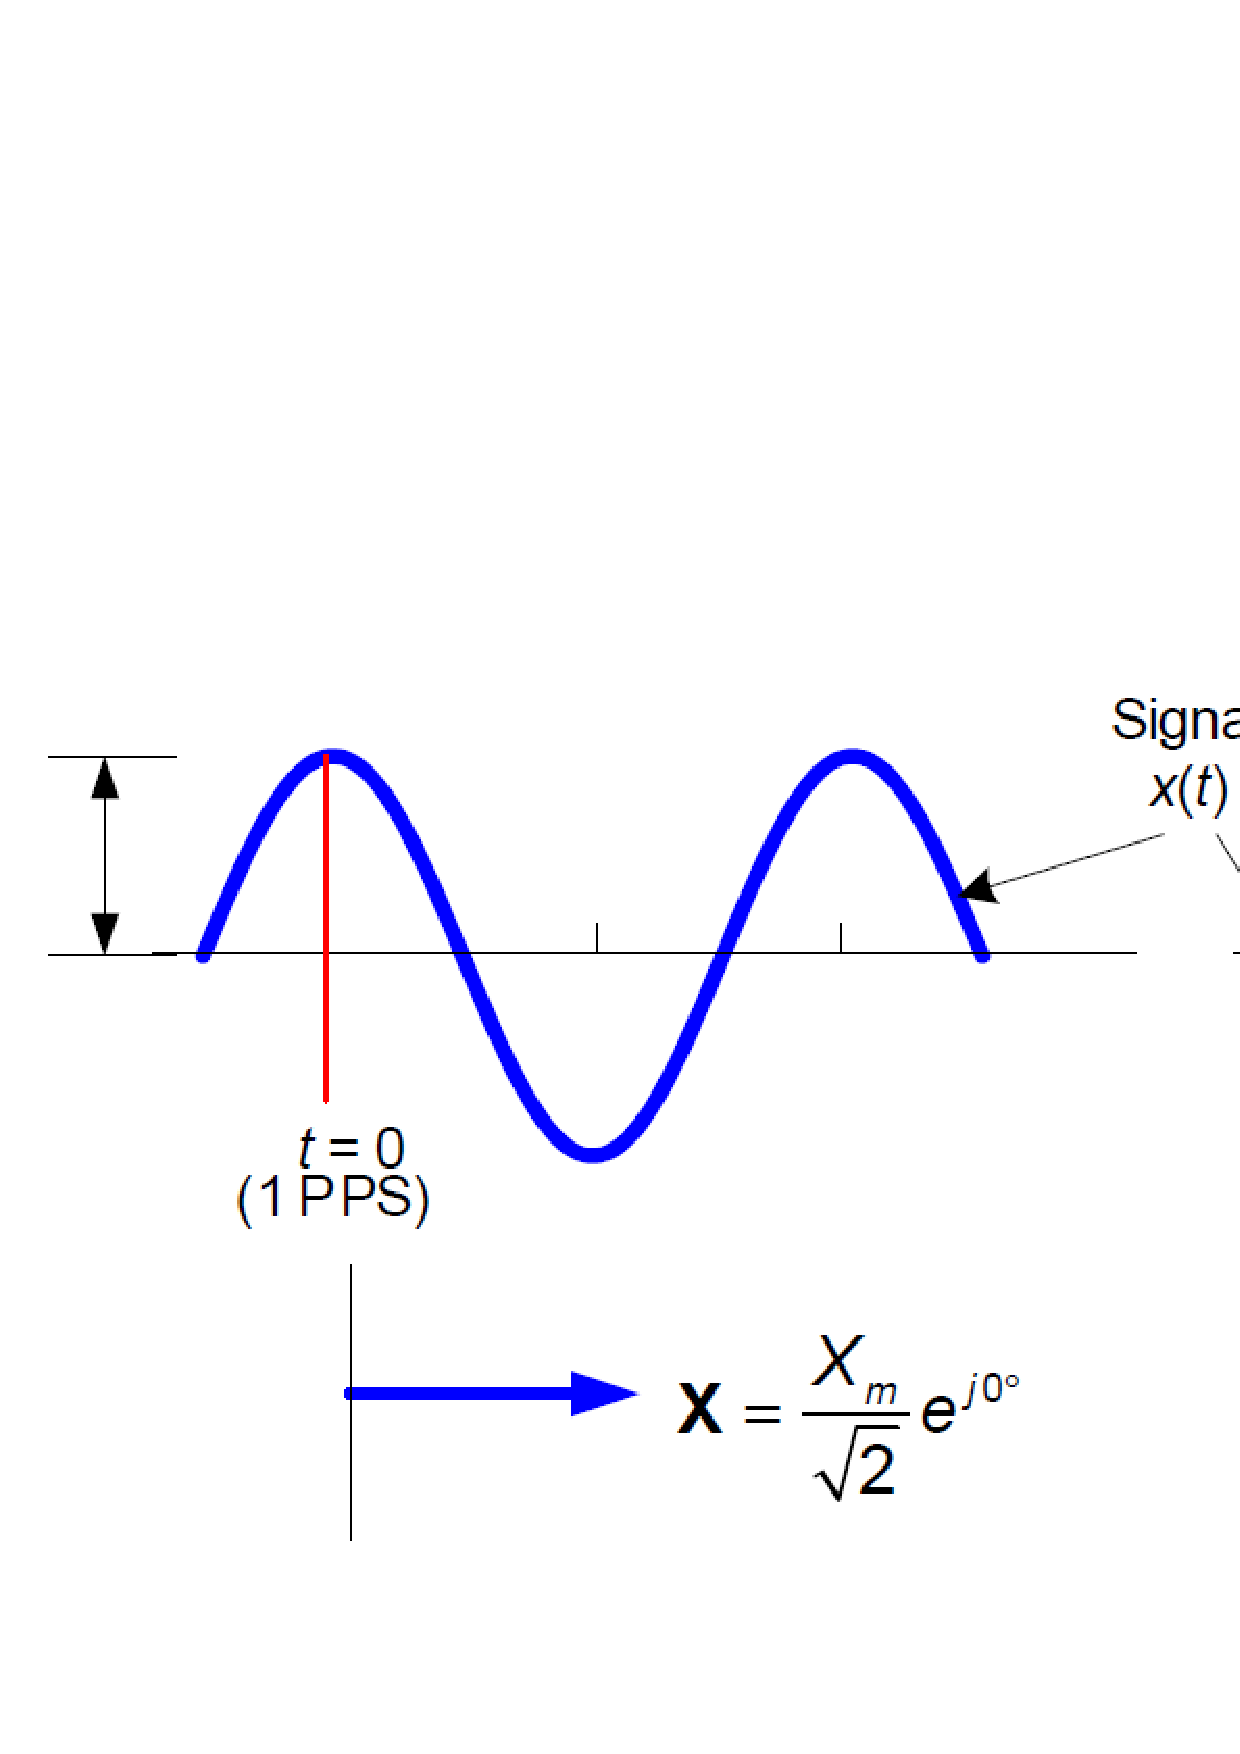
\includegraphics[ width=\textwidth]{figures/Synchrophasor-Definition.png}
    \caption[Convention for synchrophasor representation]{As presented in \Cite{schofield2018design}: Convention for synchrophasor representation.}.
    \label{fig:Synchrophasor-Definition}
  }
\end{figure}  


\subsubsection{The Synchrophasor}

    As explained in \Cite{schofield2018design}, the Synchrophasor is defind as:
\begin{equation}
    X=\frac{X_m}{\sqrt{2}}e^{j\phi}
\end{equation}
 The signal $x(t)$ is a periodic signal given by the function:


 
  \begin{equation}
      x(t) = x_mcos(\omega t + \phi )
  \end{equation}
The equations and formulae of the Synchrophasor has been modified over the years,as new editions of the standard have been published. 

\subsection{Synchrophasor Protocols}

%\hl{The introduction of Synchrophasors in the} \acrlong{pg}, 

%\subsubsection{The hhistorical background of Synchrophasors.}



As described in \cite{martin2014overview} and \cite{ali2016performance}, the communication and data exchange from the PMU to the PDC was standardised by the introduction of the IEEE 1344 standard in 1995, which was established as the standard communication protocol for synchrophasor data exchange. According to \cite{appasani2018review}, the IEEE 1344 was revised in 2001 , before the introduction of the IEEE C37.118 in 2005. The  IEEE C37.118 protocol was derived from the IEEE 1344 standard, and has undergone a number of revisions, over the years.
In \cite{martin2014overview}, \citeauthor{martin2014overview} describes the history of the 
IEEE C37.118-series of standards. The characteristics of the various generations, might be summarised as:
\begin{itemize}
 
    \item The IEEE C37.118-2005, introduced the transmission hierarchy of  \acrshort{pmu} to various levels of \acrshort{pdc}s, and super \acrshort{pdc}s.
    \item The IEEE C37.118-2011, introduced the separation of the standard into two parts:
    \begin{itemize}
    \item The IEEE C37.118-2011-1, which covers masurements and performance requirements.
    \item The IEEE C37.118-2011-2, which covers communications, and real-time transfer of data to via \acrshort{pdc}s, to the \acrshort{wams}.  
    \item The  IEEE Std. C37.118.1a-2014 is, according to \Cite{schofield2018design} an ammendment to the 2011 verisons of the standard. 
    \end{itemize}
\end{itemize}

The IEEE C37.118 series of protocols has, although not designed with security in mind, been updated with security extensions in order to ensure a trustworthy connection less vulnerable to attack on integrity and availability. 

  